\documentclass[aspectratio=169,11pt]{beamer}

% ============================================================
% PACKAGES
% ============================================================
\usepackage{graphicx}
\usepackage{tikz}
\usetikzlibrary{positioning,arrows.meta}
\usepackage{xcolor}
\usepackage{booktabs}
\usepackage{tabularx}
\usepackage{array}
\usepackage{ragged2e}
\usepackage{hyperref}

% ============================================================
% COLORS - SAME AS PHASE-I
% ============================================================
\definecolor{GEUBlue}{RGB}{20,55,105}
\definecolor{GEULightBlue}{RGB}{238,244,251}
\definecolor{GEUGrey}{RGB}{90,90,90}
\definecolor{GEULightGrey}{RGB}{245,246,248}

% ============================================================
% BEAMER SETTINGS
% ============================================================
\usetheme{default}
\setbeamertemplate{navigation symbols}{}
\setbeamertemplate{blocks}[rounded][shadow=false]

\setbeamercolor{normal text}{fg=black,bg=white}
\setbeamercolor{frametitle}{fg=GEUBlue}
\setbeamercolor{structure}{fg=GEUBlue}
\setbeamercolor{block title}{fg=GEUBlue,bg=GEULightBlue}
\setbeamercolor{block body}{fg=black,bg=GEULightBlue}

\setbeamerfont{frametitle}{size=\Large,series=\bfseries}

% ============================================================
% LOGO
% ============================================================
% Upload Graphic Era logo as graphicera_logo.png
\newcommand{\GEULogo}{graphicera_logo.png}

% ============================================================
% HEADER
% ============================================================
\setbeamertemplate{headline}{%
  \begin{tikzpicture}[remember picture,overlay]
    \node[
        anchor=north east,
        xshift=-0.30cm,
        yshift=-0.12cm
    ] at (current page.north east)
    {\includegraphics[height=0.62cm]{\GEULogo}};
  \end{tikzpicture}
  \vspace{0.72cm}
}

% ============================================================
% FRAME TITLE
% ============================================================
\setbeamertemplate{frametitle}{%
  \vspace{0.03cm}
  \insertframetitle\par
  \vspace{0.04cm}
  \textcolor{GEUBlue}{\rule{\textwidth}{0.9pt}}
  \vspace{0.03cm}
}

% ============================================================
% FOOTER
% ============================================================
\setbeamertemplate{footline}{%
  \leavevmode
  \hbox{%
  \begin{beamercolorbox}[
      wd=.82\paperwidth,
      ht=0.32cm,
      dp=0.10cm,
      leftskip=.3cm
  ]{author in head/foot}
    \tiny Department of Computer Science \& Engineering |
    Graphic Era (Deemed to be University)
  \end{beamercolorbox}%
  \begin{beamercolorbox}[
      wd=.18\paperwidth,
      ht=0.32cm,
      dp=0.10cm,
      rightskip=.3cm
  ]{date in head/foot}
    \hfill\tiny\insertframenumber/\inserttotalframenumber
  \end{beamercolorbox}}
}

% ============================================================
% CUSTOM COMMANDS
% ============================================================
\newcommand{\smallnote}[1]{%
\vspace{0.08cm}
{\scriptsize\color{GEUGrey}#1}
}

\newcommand{\placeholder}[1]{%
\textit{\color{GEUGrey}#1}
}

% ============================================================
% DOCUMENT INFORMATION
% ============================================================
\title{\textbf{Project-Based Learning}\\[2mm]\large Phase-III Evaluation}

\author{
\textbf{RouteRush: Graph-Based Order Prioritization and Delivery System}\\
Team ID: DSCPP-III-2026-T090 (404 CREW)
}

\institute{
Department of Computer Science \& Engineering\\
Graphic Era (Deemed to be University), Dehradun
}

\date{Academic Session 2026--27}

\newcommand{\todo}[1]{\textit{\color{red}#1}}

\begin{document}

\begin{frame}[plain]
\begin{tikzpicture}[remember picture,overlay]
\draw[GEUBlue,line width=3pt] (current page.north west) -- (current page.north east);
\node[anchor=north east,xshift=-0.45cm,yshift=-0.35cm] at (current page.north east) {\includegraphics[height=1.0cm]{\GEULogo}};
\node[align=center,text width=.84\paperwidth] at ([yshift=.25cm]current page.center)
{
{\color{GEUBlue}\fontsize{26}{30}\selectfont\bfseries PROJECT-BASED LEARNING}\\[3mm]
{\fontsize{18}{22}\selectfont PHASE-III FINAL EVALUATION}\\[7mm]
{\color{GEUGrey}\Large\bfseries RouteRush: Graph-Based Order Prioritization\\and Delivery System}\\[3mm]
{\color{GEUBlue}\normalsize Team ID: DSCPP-III-2026-T090 \quad (404 CREW)}
};
\node[align=center,anchor=south,yshift=.42cm] at (current page.south)
{\bfseries Department of Computer Science \& Engineering\\
Graphic Era (Deemed to be University), Dehradun\\[-1mm]
\scriptsize Academic Session 2026--27};
\end{tikzpicture}
\end{frame}

% ---------------- 2
\begin{frame}{Team \& Mentor Details}
\footnotesize
\begin{columns}[T,totalwidth=\textwidth]
\column{.48\textwidth}
\begin{block}{Team Information}
\begin{tabular}{@{}ll@{}}
\textbf{Team ID:} & DSCPP-III-2026-T090\\
\textbf{Team name:} & 404 CREW\\
\textbf{Semester:} & 3rd\\
\textbf{Section:} & \todo{XX}\\
\textbf{Domain:} & Data structures, C++ systems
\end{tabular}
\end{block}
\column{.48\textwidth}
\begin{block}{Team Members}
1.\quad Sharma Sundram -- 2028872 (lead)\\
2.\quad Agarwal Samriddhi -- 2028482\\
3.\quad Kumari Arya -- 2028665\\
4.\quad Sirohi Ishita -- 2028730
\end{block}
\end{columns}
\vspace{2mm}
\begin{block}{Mentor}
Dr. Pawan Kumar Mishra\hfill\textbf{Interactions:} 3
\end{block}
\vfill
\end{frame}

% ---------------- 3
\begin{frame}{Project Abstract \& Problem Statement}
\footnotesize
\begin{block}{Project Abstract}
\small RouteRush ranks orders with an aging priority queue, reserves stock, plans picking routes on a warehouse graph (Dijkstra, nearest-neighbour, 2-opt), assigns bikes, vans and trucks, and logs deliveries. It is C++17 with only the STL, plus a terminal menu and a local web dashboard with a 3D replay.
\end{block}
\begin{block}{Problem Statement}
\small Serving orders in arrival order makes urgent orders wait and pickers walk long routes. Does priority with aging plus planned routes help, and what does it cost lower-priority orders?
\end{block}
\textbf{\color{GEUBlue}Target Users}
\begin{itemize}\itemsep2pt
    \item Small-warehouse dispatchers (mixed urgency)
    \item Local use; synthetic data; benefit and trade-off both shown
\end{itemize}
\end{frame}

% ---------------- 4
\begin{frame}{Objectives \& Final Deliverables}
\footnotesize
\begin{columns}[T,totalwidth=\textwidth]
\column{.48\textwidth}
\textbf{\color{GEUBlue}Finalized Objectives}
\begin{enumerate}\itemsep3pt
    \item Rank orders by priority without starving the rest (aging).
    \item Reserve stock all-or-nothing so inventory never goes negative.
    \item Plan picking routes on a graph and compare against naive order.
    \item Assign the cheapest fitting vehicles from a fleet.
    \item Show the trade-offs honestly against a FIFO baseline.
\end{enumerate}
\column{.48\textwidth}
\textbf{\color{GEUBlue}Final Deliverables}
\begin{itemize}\itemsep3pt
    \item C++17 backend, terminal menu and local web dashboard
    \item Source code on GitHub (STL only)
    \item CSV data: layout, products, orders, results
    \item 68 tests (793 checks) and benchmarks
    \item README, architecture, data-structure, testing and benchmark documents
\end{itemize}
\end{columns}
\vfill
\end{frame}

% ---------------- 5
\begin{frame}{Phase-I \& Phase-II Feedback Incorporated}
\scriptsize
\begin{center}
\renewcommand{\arraystretch}{1.35}
\begin{tabularx}{.96\textwidth}{@{}p{2.1cm}X X@{}}
\toprule
\textbf{Phase} & \textbf{Feedback / Suggestion} & \textbf{Action Taken}\\
\midrule
Phase-I & \todo{Copy from your Phase-I evaluation sheet} & \todo{What changed}\\
Phase-I & \todo{Copy from your Phase-I evaluation sheet} & \todo{What changed}\\
Phase-II & \todo{Copy from your Phase-II evaluation sheet} & \todo{What changed}\\
Phase-II & \todo{Copy from your Phase-II evaluation sheet} & \todo{What changed}\\
\bottomrule
\end{tabularx}
\end{center}
\vfill
\begin{block}{Final Improvement}
From a terminal-only simulation to a tested system with a menu, a local web dashboard (orders, stock, 3D playback, policy comparison, map) and a baseline comparison that reports both gains and costs.
\end{block}
\end{frame}

% ---------------- 6
\begin{frame}{Final System Architecture}
\footnotesize
\begin{center}
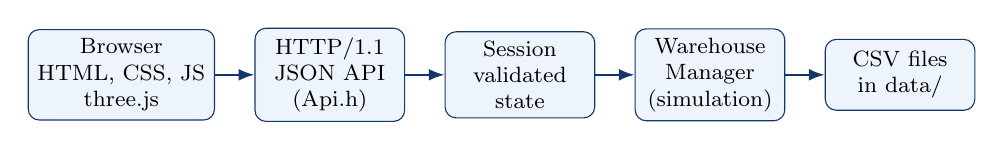
\begin{tikzpicture}[
node distance=5mm,
box/.style={rectangle,rounded corners,draw=GEUBlue,fill=GEULightBlue,minimum width=1.9cm,minimum height=9mm,align=center,font=\footnotesize},
arrow/.style={-{Latex[length=2mm]},thick,draw=GEUBlue}]
\node[box] (a) {Browser\\HTML, CSS, JS\\three.js};
\node[box,right=of a] (b) {HTTP/1.1\\JSON API\\(Api.h)};
\node[box,right=of b] (c) {Session\\validated\\state};
\node[box,right=of c] (d) {Warehouse\\Manager\\(simulation)};
\node[box,right=of d] (e) {CSV files\\in data/};
\draw[arrow] (a)--(b); \draw[arrow] (b)--(c); \draw[arrow] (c)--(d); \draw[arrow] (d)--(e);
\end{tikzpicture}
\end{center}
\vspace{2mm}
\begin{columns}[T,totalwidth=\textwidth]
\column{.48\textwidth}
\textbf{\color{GEUBlue}Major Components}
\begin{itemize}\itemsep2pt
    \item OrderQueue (heap with aging), Inventory on a HashMap
    \item Graph, Dijkstra, RoutePlanner (naive, NN, 2-opt)
    \item Fleet with Bike, Van and Truck
    \item Session, Api, HttpServer, static file server
\end{itemize}
\column{.48\textwidth}
\textbf{\color{GEUBlue}System Flow}
\begin{itemize}\itemsep2pt
    \item Input: order form or \texttt{orders.csv}
    \item Processing: rank, check stock, plan route, pick vehicles
    \item Storage: CSV files; every run replays on a fresh copy
    \item Output: records, metrics and per-order routes for the 3D replay
\end{itemize}
\end{columns}
\vfill
\end{frame}

% ---------------- 7
\begin{frame}{Final Technology Stack}
\footnotesize
\begin{columns}[T,totalwidth=\textwidth]
\column{.48\textwidth}
\begin{block}{Software / Technologies}
\begin{itemize}\itemsep2pt
    \item Programming: C++17 (backend), JavaScript (front end)
    \item Framework: none; hand-written HTTP layer
    \item Database: CSV files
    \item Libraries: STL only; three.js r128 for 3D in the browser
    \item OS/Platform: Windows (Winsock) and Linux (POSIX sockets)
\end{itemize}
\end{block}
\column{.48\textwidth}
\begin{block}{Development Infrastructure}
\begin{itemize}\itemsep2pt
    \item Compiler: GCC (WinLibs) with \texttt{-std=c++17}
    \item Version Control: Git/GitHub
    \item Testing: own TEST/CHECK framework, Node for page logic
    \item Build: Makefile and \texttt{run.bat}
    \item Deployment: GitHub repository
\end{itemize}
\end{block}
\end{columns}
\vfill
\end{frame}

% ---------------- 8
\begin{frame}{Implementation of PBL Course Concepts}
\scriptsize
\begin{center}
\renewcommand{\arraystretch}{1.25}
\begin{tabularx}{.96\textwidth}{@{}>{\bfseries}p{2.8cm}X p{2.8cm}@{}}
\toprule
Course & Concepts Actually Implemented & Project Module\\
\midrule
Data Structures in C &
Binary heap with aging key; hash table with chaining and rehash; graph as adjacency list; Dijkstra; nearest-neighbour and 2-opt heuristics &
OrderQueue, HashMap, Inventory, Graph, RoutePlanner\\
OOPs with C++ &
Classes and encapsulation, inheritance and virtual functions (Bike, Van, Truck), templates (HashMap), STL containers, RAII, const-correctness &
Vehicle, Fleet, Session, HttpServer\\
\bottomrule
\end{tabularx}
\end{center}
\vfill
\begin{center}
\colorbox{GEULightBlue}{\parbox{.88\textwidth}{\centering
\textbf{Semester 3:} Data Structures + OOPs with C++. Each concept above has a unit test and can be shown in the code.}}
\end{center}
\end{frame}

% ---------------- 9
\begin{frame}{Module-Wise Final Implementation}
\scriptsize
\begin{center}
\renewcommand{\arraystretch}{1.05}
\begin{tabularx}{.96\textwidth}{@{}p{2.4cm}X p{2.0cm}p{1.7cm}@{}}
\toprule
\textbf{Module} & \textbf{Implementation} & \textbf{Responsible} & \textbf{Status}\\
\midrule
Pipeline, fleet &
WarehouseManager event simulation, vehicle choice, delivery log, metrics & Sundram & Completed\\
Session, API, server &
Validated state, JSON API, threaded local HTTP server, safe static files & Sundram & Completed\\
Dashboard &
7 pages: orders, stock, 3D simulation, comparison, map, route finder & Sundram, Arya & Completed\\
Data structures &
HashMap, Inventory (atomic reserve), OrderQueue with aging, HTTP parsing & Samriddhi & Completed\\
Graph, routing &
Graph, Dijkstra, naive/NN/2-opt, layout and 3D scene logic & Arya & Completed\\
Storage, tests &
CSV stores, test framework, 68 tests, benchmarks & Ishita & Completed\\
\bottomrule
\end{tabularx}
\end{center}
\vspace{2mm}
\begin{center}
\colorbox{GEULightBlue}{\parbox{.8\textwidth}{\centering
\textbf{Planned scope completed.} Not built: live (non-replay) mode, login, a real database.}}
\end{center}
\vfill
\end{frame}

% ---------------- 10
\begin{frame}{Working System / Prototype Demonstration}
\footnotesize
\begin{columns}[T,totalwidth=\textwidth]
\column{.43\textwidth}
\textbf{\color{GEUBlue}Major Working Features}
\begin{itemize}\itemsep3pt
    \item Add, filter and remove orders; restock products
    \item Simulation Lab: pickers and vehicles follow the real routes in 3D
    \item Compare: priority and aging vs FIFO baseline
    \item Warehouse Map: node details and a Dijkstra route finder
    \item Terminal menu and CSV output
\end{itemize}
\column{.53\textwidth}
\begin{block}{System Screenshot / Output}
\centering\vspace{11mm}
\todo{Insert a screenshot of the Simulation Lab page}
\vspace{11mm}
\end{block}
\end{columns}
\vfill
\end{frame}

% ---------------- 11
\begin{frame}{Data / Database / Backend Implementation}
\footnotesize
\begin{columns}[T,totalwidth=\textwidth]
\column{.48\textwidth}
\textbf{\color{GEUBlue}Data / Database}
\begin{itemize}\itemsep3pt
    \item Source: \texttt{layout.csv}, \texttt{products.csv}, \texttt{orders.csv} (synthetic orders; approximate road distances)
    \item Demo graph: GEU warehouse + 3 Dehradun stops, 13 edges, 6 products
    \item Entities: node, edge, product, order line, order, vehicle, record
    \item Retrieval: loaded once into memory; HashMap by product id
    \item Validation: bad CSV lines skipped and counted; API checks every field
\end{itemize}
\column{.48\textwidth}
\textbf{\color{GEUBlue}Backend / Core Logic}
\begin{itemize}\itemsep3pt
    \item Each run replays all orders on a fresh inventory and fleet
    \item API: state, compare, order, product, restock, run, reset
    \item Rank = priority score plus aging; heap pop per tick
    \item Security: loopback only, path-checked static files, no login
    \item Errors: clear rejection reasons; a rejected order leaves state unchanged
\end{itemize}
\end{columns}
\vfill
\end{frame}

% ---------------- 12
\begin{frame}{Testing \& Validation}
\scriptsize
\begin{center}
\renewcommand{\arraystretch}{1.05}
\begin{tabularx}{.96\textwidth}{@{}p{2.0cm}X X p{1.0cm}@{}}
\toprule
Test Type & Expected Result & Observed Result & Status\\
\midrule
Unit (data structures) & Heap order, rehash of 5000 keys, atomic stock reserve & All checks pass & Pass\\
Unit (graph, routes) & NN beats naive on a known case; reported distance equals walked path & Pass; 2-opt $\le$ NN on 60 random cases & Pass\\
Integration & Rejections leave state untouched; deadlines and busy vehicles handled & Pass (pipeline tests) & Pass\\
API and HTTP & Bad input rejected; unknown path gives 404; path traversal refused & Pass (15 tests) & Pass\\
Page logic (Node) & Layout, playback and Dijkstra match the C++ output & Pass, run outside the repo & Pass\\
\bottomrule
\end{tabularx}
\end{center}
\begin{block}{Validation Summary}
68 tests, 793 checks, 0 failed. Not covered: huge layouts, CSV fuzzing, browser rendering of the 3D scene.
\end{block}
\end{frame}

% ---------------- 13
\begin{frame}{Results \& Performance Analysis}
\footnotesize
\begin{columns}[T,totalwidth=\textwidth]
\column{.50\textwidth}
\textbf{\color{GEUBlue}Key Results (demo data, 8 orders)}
\begin{itemize}\itemsep3pt
    \item URGENT wait: 82.0 $\to$ 17.5 ticks
    \item Late orders: 1 $\to$ 0; makespan 304 $\to$ 277
    \item Cost: EXPRESS wait 70.5 $\to$ 92.0 (+30\%), NORMAL 67.7 $\to$ 102.3 (+51\%)
    \item Benchmark (300 orders, 8x8 grid): NN picks 33\% shorter than naive, 2-opt 38\%
    \item Hash map vs linear scan: about 1000x faster at 100k products
\end{itemize}
\column{.46\textwidth}
\begin{block}{Average wait by priority (ticks)}
\centering
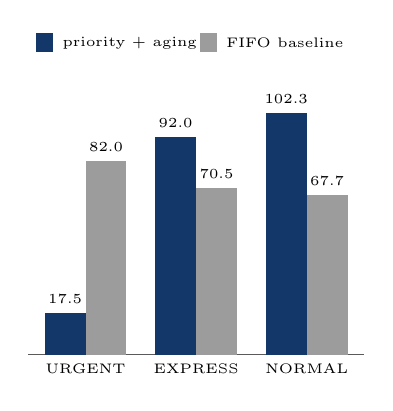
\begin{tikzpicture}[x=0.52cm,y=0.030cm,font=\tiny]
\draw[GEUGrey] (0,0)--(8.2,0);
\foreach \x/\a/\b/\l in {0.4/17.5/82.0/URGENT,3.1/92.0/70.5/EXPRESS,5.8/102.3/67.7/NORMAL}{
  \fill[GEUBlue] (\x,0) rectangle (\x+1,\a); \fill[GEUGrey!60] (\x+1,0) rectangle (\x+2,\b);
  \node[above] at (\x+0.5,\a) {\a}; \node[above] at (\x+1.5,\b) {\b};
  \node[below] at (\x+1,0) {\l};}
\fill[GEUBlue] (0.2,128) rectangle (0.6,136); \node[right] at (0.6,132) {priority + aging};
\fill[GEUGrey!60] (4.2,128) rectangle (4.6,136); \node[right] at (4.6,132) {FIFO baseline};
\end{tikzpicture}
\end{block}
\end{columns}
\vfill
\end{frame}

% ---------------- 14
\begin{frame}{GitHub Repository \& Development Evidence}
\footnotesize
\begin{columns}[T,totalwidth=\textwidth]
\column{.45\textwidth}
\textbf{\color{GEUBlue}Repository Details}
\begin{itemize}\itemsep3pt
    \item Repo: \texttt{sundramsharma-2006/}\\\texttt{RouteRush-Graph-Based-Order-}\\\texttt{Prioritization-Delivery-System}
    \item Branch: main
    \item README.md: usage, ownership table
    \item Contributors: \todo{confirm all four}
    \item Documentation: \texttt{docs/} (4 files)
\end{itemize}
\column{.51\textwidth}
\textbf{\color{GEUBlue}Development Evidence}
\begin{itemize}\itemsep3pt
    \item Phase-III commit plan: 10 commits split by owner
    \item Each member commits their own files
    \item \todo{Commit count and history: fill after pushing}
\end{itemize}
\end{columns}
\vfill
\begin{center}
\colorbox{GEULightBlue}{\parbox{.88\textwidth}{\centering
\textbf{Requirement:} all members must be contributors and individual activity must be visible in the history.}}
\end{center}
\end{frame}

% ---------------- 15
\begin{frame}{Individual Contribution}
\scriptsize
\begin{center}
\renewcommand{\arraystretch}{1.05}
\begin{tabularx}{.96\textwidth}{@{}p{1.8cm}p{1.9cm}X p{1.5cm}@{}}
\toprule
Member & Role & Final Technical Contribution & Commits\\
\midrule
Sundram Sharma & Lead; pipeline, API, UI & Vehicle, Fleet, WarehouseManager, Session, Api, HttpServer, Menu, dashboard pages and styling, build scripts & \todo{XX}\\
Samriddhi Agarwal & Data structures & HashMap, Inventory (atomic reserve), OrderQueue with aging, HTTP parsing, static file safety & \todo{XX}\\
Arya Kumari & Graph and routing & Graph, Dijkstra, RoutePlanner (NN, 2-opt), warehouse layouts, layout and 3D scene code & \todo{XX}\\
Ishita Sirohi & Storage and testing & CSV stores, test framework, API tests, benchmarks, data files & \todo{XX}\\
\bottomrule
\end{tabularx}
\end{center}
\vspace{2mm}
\begin{block}{Individual Evaluation}
Every member must be able to explain, demonstrate and defend their own files in the viva.
\end{block}
\end{frame}

% ---------------- 16
\begin{frame}{Challenges, Limitations \& Lessons Learned}
\footnotesize
\begin{columns}[T,totalwidth=\textwidth]
\column{.48\textwidth}
\textbf{\color{GEUBlue}Challenges \& Solutions}
\begin{itemize}\itemsep3pt
    \item Old GCC 6.3 failed on C++17: installed a current GCC and put it first on PATH
    \item No sockets in the STL, and Windows differs from Linux: one header for both; thread per connection with one lock
    \item Trade-off visible: priority hurts EXPRESS and NORMAL waits, so we report it
\end{itemize}
\vspace{1mm}
\textbf{\color{GEUBlue}Current Limitations}
\begin{itemize}\itemsep2pt
    \item Replay, not live; CSV, not a database
    \item Synthetic data; heuristics are not optimal
\end{itemize}
\column{.48\textwidth}
\textbf{\color{GEUBlue}Technical Learning}
\begin{itemize}\itemsep3pt
    \item A heap needs an aging rule or low priority starves
    \item Heuristics (NN, 2-opt) need a baseline to prove value
    \item Concurrency needs a lock even for a local server
\end{itemize}
\vspace{1mm}
\textbf{\color{GEUBlue}Team Learning}
\begin{itemize}\itemsep2pt
    \item Splitting by header files with tests per owner
    \item Each owner writes tests for their own module
\end{itemize}
\end{columns}
\end{frame}

% ---------------- 17
\begin{frame}{Final Outcomes, Applications \& Future Scope}
\footnotesize
\begin{columns}[T,totalwidth=\textwidth]
\column{.32\textwidth}
\textbf{\color{GEUBlue}Final Outcomes}
\begin{itemize}\itemsep3pt
    \item Working C++ system and dashboard
    \item 68 tests, 793 checks passing
    \item Measured comparison with its costs
\end{itemize}
\column{.32\textwidth}
\textbf{\color{GEUBlue}Applications}
\begin{itemize}\itemsep3pt
    \item Dispatch teaching and training tool
    \item Policy what-if analysis for small warehouses
    \item Base for a real order system
\end{itemize}
\column{.32\textwidth}
\textbf{\color{GEUBlue}Future Scope}
\begin{itemize}\itemsep3pt
    \item Live mode and a real database
    \item Real or public order data
    \item Better routing, several pickers
\end{itemize}
\end{columns}
\vspace{5mm}
\begin{block}{Tangible Project Outcome}
A tested working prototype with source code, a local web dashboard, benchmarks and documents. It has not been deployed or validated on real warehouse data.
\end{block}
\end{frame}

% ---------------- 18
\begin{frame}{References \& Project Resources}
\footnotesize
\begin{columns}[T,totalwidth=\textwidth]
\column{.53\textwidth}
\textbf{\color{GEUBlue}References}
\begin{enumerate}\itemsep3pt
    \item E. W. Dijkstra, ``A note on two problems in connexion with graphs,'' Numerische Mathematik, 1959.
    \item G. A. Croes, ``A method for solving traveling-salesman problems,'' Operations Research, 1958 (2-opt).
    \item cppreference.com: C++17 standard library.
    \item three.js documentation, r128.
    \item Project \texttt{docs/} and benchmark output (synthetic).
\end{enumerate}
\column{.43\textwidth}
\textbf{\color{GEUBlue}Project Resources}
\begin{itemize}\itemsep3pt
    \item GitHub: github.com/sundramsharma-2006/RouteRush-Graph-Based-Order-Prioritization-Delivery-System
    \item Dataset: \texttt{data/} (synthetic)
    \item Documentation: \texttt{docs/}, README.md
\end{itemize}
\vfill
\begin{center}
\colorbox{GEUBlue}{\parbox{.82\textwidth}{\centering\color{white}\Large\textbf{Thank You}\\[1mm]\normalsize Questions \& Discussion}}
\end{center}
\end{columns}
\end{frame}

\end{document}
